\chapter{Evaluation}
\label{chap:evaluation}
Biohadoops purpose is to facilitate the implementation of parallel algorithms on Hadoop. It is expected that the execution time of an algorithm reduces if it is parallelized (assuming the algorithm is suitable for parallelization). That means the speedup increases when computational resources are added. To verify this assumption, two bio-inspired optimization algorithms are parallelized using Biohadoop. Their parallel parts are executed on Biohadoop workers. The execution times of the algorithms are measured on a Hadoop cluster. Then, the speedups are calculated based on those execution times. The speedups demonstrate if the algorithm execution times benefit from the parallelization.

The rest of this chapter is structured as follows: section \ref{chap:evaluation:cluster} provides information about the cluster used for the benchmarks. Section \ref{chap:evaluation:testproblems} describes the benchmarked test problems. The benchmark results are presented in section \ref{chap:evaluation:benchmarks} together with a check for their correctness. Section \ref{chap:evaluation:influence} gives a discussion of the most notable factors that influence the execution time. The speedup calculations can be found in section \ref{chap:evaluation:speedup}. Finally, section \ref{chap:evaluation:comparison} compares the execution times of Biohadoop parallelellized algorithms to their standalone implementations.

\section{Cluster Hardware}
\label{chap:evaluation:cluster}
All benchmarks are performed on a Hadoop cluster with 6 identical computers. Each machine has the following specifications:

\begin{itemize}
  \item Intel Core2 Duo CPU E8200 @ \unit[2.66]{GHz} (2$\times$\unit[2.66]{GHz}, no hyperthreading)
  \item \unit[6]{MB} shared L2 cache, \unit[32]{KB} L1 data cache, \unit[32]{KB} L1 instruction cache
  \item \unit[4]{GB} (2$\times$\unit[2]{GB}) DDR2 RAM @ \unit[667]{MHz}
  \item \unit[64]{Bit} Ubuntu Linux 14.04.1 LTS with kernel 3.13.0-37
\end{itemize}

The computers are directly connected to the same Switch through a 1Gb (Gigabit) Ethernet network.

\section{Test Problems}
\label{chap:evaluation:testproblems}
NSGA-II and a simple GA are the implemented bio-inspired optimization algorithms used for the benchmarks. They can handle different numbers objectives. While NSGA-II is used to solve the MOPs in section \ref{chap:evaluation:zdt3}, a simple GA is used to solve the SOPs in section \ref{chap:evaluation:tiledmul}.

\subsection{ZDT-3}
\label{chap:evaluation:zdt3}
The first optimization algorithm is NSGA-II, used to find optimal solutions for the Zitzler–Deb–Thiele's function nr. 3 \cite{zitzler2000comparison}. ZDT-3 is part of the well known ZDT family of MOPs. It was chosen because of its discontinuous optimal Pareto Front (see figure \ref{fig:zdt3}) that can pose problems to simpler optimization strategies, e.g., gradient based algorithms. The expected outcome is to find an approximation to the optimal Pareto Front.

\begin{figure}
  \centering
  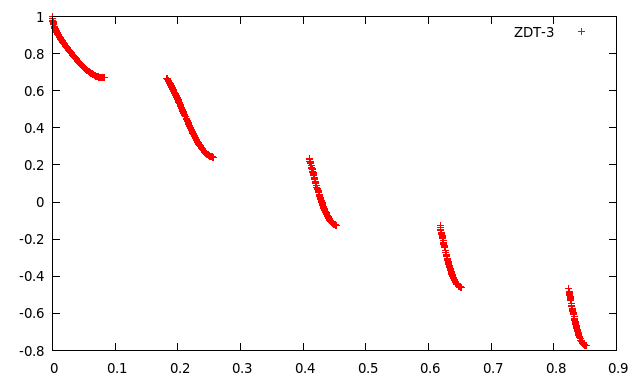
\includegraphics[width=110mm,natwidth=640,natheight=384]{zdt3.png}
  \caption[Optimal Pareto Front for ZDT-3]{Optimal Pareto Front for ZDT-3}
  \label{fig:zdt3}
\end{figure}

The implementation uses Biohadoop workers to create and evaluate the offsprings. Simulated Binary Crossover (SBX) and Parameter based mutation \cite{deb2000efficient} are used for the offspring creation. The fitness is computed using the ZDT-3 function. The selection of the fittest individuals for the next population is based on ranking and crowding distance and is performed on the master.

The ZDT-3 benchmark instances are executed with genome sizes of 10, 100, 1000 and 10000. The genome size influences two properties of the ZDT-3 benchmark instances. First, increasing the number of genomes also increases the computation effort for the workers that generate new offsprings and compute their fitness. This is due to the fact that new individuals are generated using parent genomes and that the ZDT-3 algorithm, used for the fitness computation, loops over all genomes. Second, the genome size influences the amount of data that has to be transferred between the master and the workers. Each worker repeatedly receives two parent individuals and returns an offspring and its computed fitness. The amount of data sent between master and workers is, therefore, related to the gnome size of each individual.

\subsection{Tiled Matrix Multiplication}
\label{chap:evaluation:tiledmul}
The second benchmark implements a GA to solve the SOP for finding optimal tile sizes for the tiled matrix multiplication (TMM). The objective is to minimize the execution time for a matrix multiplication. The expected outcome are tile sizes that minimizes the TMM execution time.

A matrix multiplication can be performed in different ways. The most obvious one is the standard algorithm:
\begin{lstlisting}
for i = 1 to n
  for j = 1 to m
    for k = 1 to l
      C(i,j) = C(i,j) + A(i,k) * B(k,j)
\end{lstlisting}

The matrix multiplication can be improved by loop tiling \cite{wolfe1989more}. The computation is performed on smaller blocks (tiles) of the matrices:
\begin{lstlisting}
for i0 = 1 to n, step blocksize_i
  for j0 = 1 to m, step blocksize_j
    for k0 = 1 to l, step blocksize_k
      for i = i0 to min(i0 + blocksize_i, n)
        for j = j0 to min(j0 + blocksize_j, m)
          for k = k0 to min(k0 + blocksize_k, l)
            C(i,j) = C(i,j) + A(i,k) * B(k,j)
\end{lstlisting}

If the blocks are small enough they fit into the L1 CPU cache which results in a speedup. Tests with a matrix size of 1024$\times$1024 were performed on a single computer of the test cluster to demonstrate the advantages of TMM. Table \ref{table:mm_comparison} shows that suitable tile sizes can reduce the execution times for a tiled matrix multiplication. The results show also that bad tile sizes increase the execution time drastically. Therefore, one needs to find good tile sizes to profit from TMM.

\begin{table}
  \centering
  \caption{Execution times for 1024$\times$1024 matrix multiplications}
  \begin{tabular}{lrr}\toprule[2pt]
    Setting & execution time [s] \\ \midrule
    Standard algorithm & 11.384 \\
    TMM, tile size $i=j=k=1$ & 25.683 & \\
    TMM, tile size $i=j=k=32$ & 2.669 &  \\
  \end{tabular}
  \label{table:mm_comparison}
\end{table}

An optimization algorithm can be used to find the (near) optimal tile sizes for the different loops. In this case, the optimization is done using a GA. The implementation uses Biohadoops workers to create and evaluate an offspring. For the offspring creation, Simulated Binary Crossover (SBX) and Parameter based mutation are used. The fitness is computed as the time it takes to multiply two matrices using a given tile size. The selection of the fittest individuals for the next population is performed on the master.

The TMM benchmarks are executed with matrix sizes of 128$\times$128 and 256$\times$256. The matrix size influences the number of computations that need to be performed for a full matrix multiplication and, therefore, also influences the execution time. In contrast to ZDT-3, the matrix size has no impact on the amount of data transferred between the master and the workers. The matrices are part of the ``initial data'' (see chapter \ref{chap:impl:worker}) and, hence, transferred exactly once to every worker. The task data consists of two parent individuals that are transferred from the master to the workers to create a new offspring and compute its fitness. The data transferred from a worker to the master contains the offspring and its computed fitness value. Each individual consists of its tile sizes for $i$, $j$ and $k$.

\subsection{Settings}
All benchmarks are executed on the cluster described in section \ref{chap:evaluation:cluster}. They have the following settings in common:
\begin{itemize}
  \item The number of iterations is set to 250.
  \item The population size is set to 100.
  \item The distribution index $n_c$ for the SBX crossover is set to 20.
  \item The distribution index $n_m$ for the mutation is set to 20.
  \item The mutation probability for each offspring value is set to $1/n$, i.e., on average one offspring value is mutated.
\end{itemize}

Parallel benchmarks are executed with different problem sizes and different numbers of workers. Standalone sequential benchmarks, used for comparison with the parallel results in section \ref{chap:evaluation:comparison}, are executed with different problem sizes only. It makes no sense to vary the worker size for a sequential benchmark.

\section{Biohadoop Benchmarks}
\label{chap:evaluation:benchmarks}
The benchmark results presented in this section show the algorithm execution times (AETs) for the test problems that were parallelized using Biohadoop. It is expected that the AET of a test problem reduces when the number of parallel workers increases.

Before the presentation of the benchmark results, a definition of AET is given for clarification. Then, the benchmark results are presented. Afterwards, the output of the benchmarks, i.e., the optimization results, are checked for correctness.

\subsection{Definition of Algorithm Execution Time}
\label{chap:evaluation:exec-definition}
The full execution time of an algorithm running on top of Biohadoop is composed of the time Biohadoop needs to start up as a Hadoop application and the time spent in the algorithms \texttt{run} method. The time spent in the algorithms \texttt{run} method is from here on defined as AET. Figure \ref{fig:execution-times} demonstrates this concept.

\begin{figure}
  \centering
  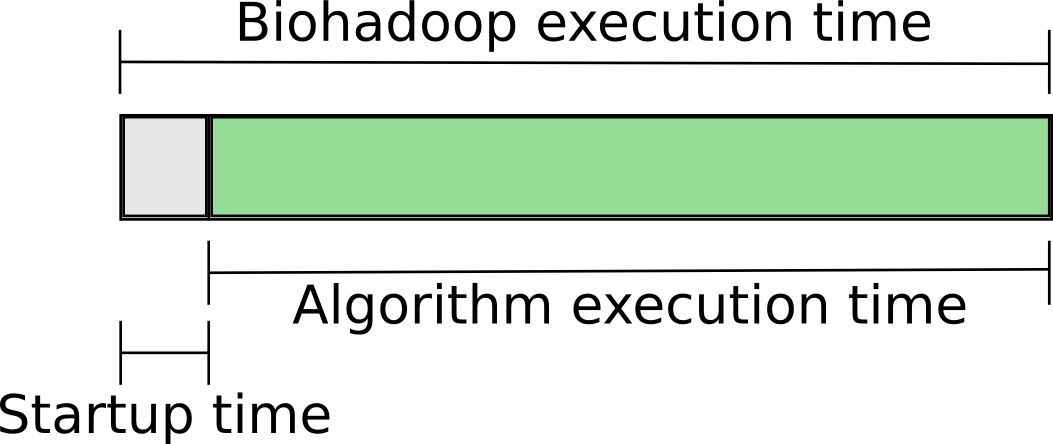
\includegraphics[width=70mm,natwidth=1053,natheight=444]{execution-times.png}
  \caption[Division of Biohadoop execution times]{Biohadoop execution times are composed of start up times and algorithm execution times}
  \label{fig:execution-times}
\end{figure}

The distinction between start up time and AET is made because the main part of the start up time is spent between the application submission to Hadoop and the beginning of its execution. It is not possible to predict when an application is executed by Hadoop as it depends on different factors like the available cluster resources. To minimize the impact of this uncertainty, the following benchmark measurements are based on AET, without the application start up time.

In contrast, the definition of AET for a program that doesn't use Biohadoop is given as the execution time of the Java program. This definition applies to the standalone sequential implementations in section \ref{chap:evaluation:comparison}, which have no Hadoop startup time.

\subsection{Benchmark results}
The results presented in this section reflect the AET for the test problems of section \ref{chap:evaluation:testproblems}. The test problems are parallelized using Biohadoop and its task system. The parallel parts are executed on Biohadoop workers.

The benchmarks are performed with worker sizes ranging from 1 to 15. Each benchmark is repeated five times to improve the reliability of the results. This gives a total of 300 benchmark runs for ZDT-3 (4 genome sizes $\times$ 15 worker setting $\times$ 5 repetitions) and 150 benchmark runs for TMM (2 tile sizes $\times$ 15 worker settings $\times$ 5 repetitions). The AET for the benchmarks are presented in fig. \ref{fig:nsga_250_100_10} to \ref{fig:nsga_250_100_10000} for the ZDT-3 test problem. Fig. \ref{fig:tiledmul_250_100_128x128} and \ref{fig:tiledmul_250_100_256x256} show the results for the TMM benchmarks.

\begin{figure}
  \centering
  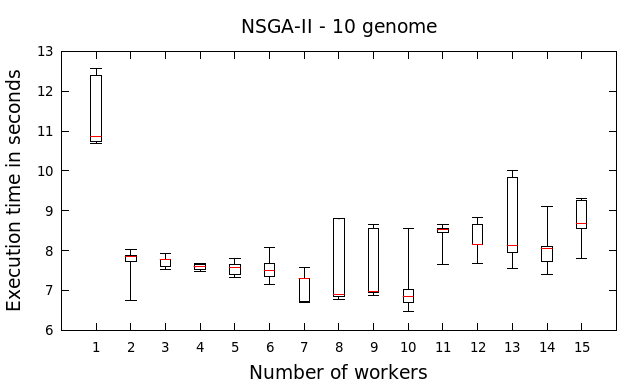
\includegraphics[width=90mm,natwidth=640,natheight=384]{nsgaii_250_100_10.png}
  \caption[ZDT-3 execution times for a genome size of 10]{ZDT-3 execution times for a genome size of 10}
  \label{fig:nsga_250_100_10}
\end{figure}
\begin{figure}
  \centering
  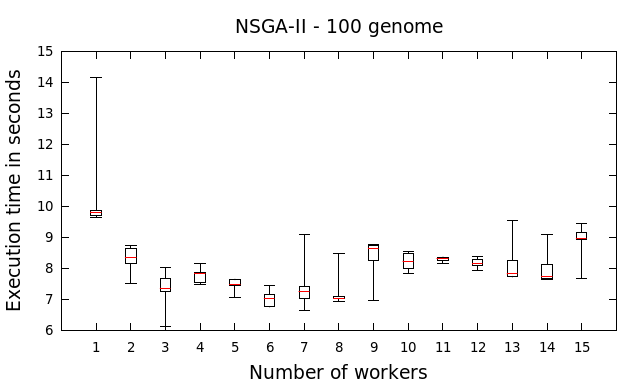
\includegraphics[width=90mm,natwidth=640,natheight=384]{nsgaii_250_100_100.png}
  \caption[ZDT-3 execution times for a genome size of 100]{ZDT-3 execution times for a genome size of 100}
  \label{fig:nsga_250_100_100}
\end{figure}
\begin{figure}
  \centering
  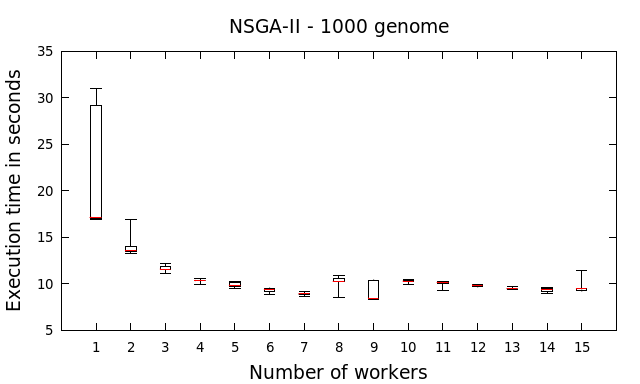
\includegraphics[width=90mm,natwidth=640,natheight=384]{nsgaii_250_100_1000.png}
  \caption[ZDT-3 execution times for a genome size of 1000]{ZDT-3 execution times for a genome size of 1000}
  \label{fig:nsga_250_100_1000}
\end{figure}
\begin{figure}
  \centering
  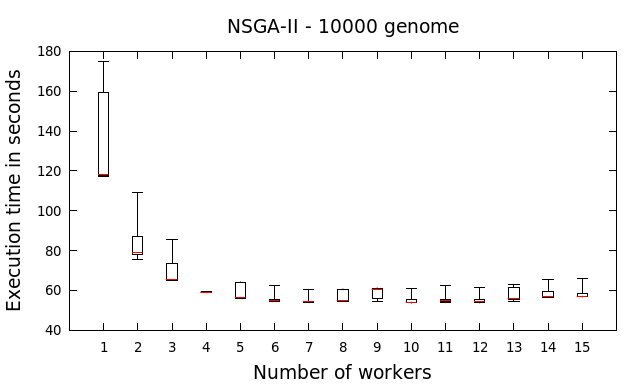
\includegraphics[width=90mm,natwidth=640,natheight=384]{nsgaii_250_100_10000.png}
  \caption[ZDT-3 execution times for a genome size of 10000]{ZDT-3 execution times for a genome size of 10000}
  \label{fig:nsga_250_100_10000}
\end{figure}

\begin{figure}
  \centering
  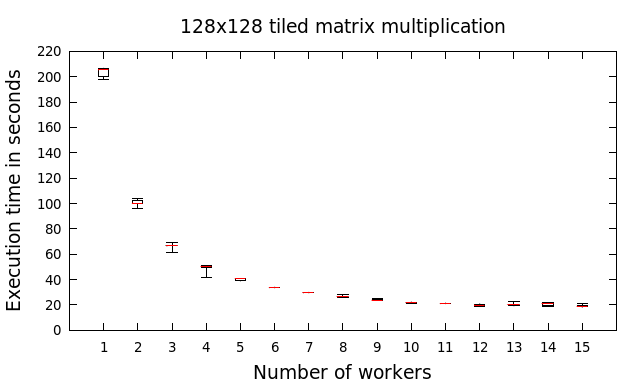
\includegraphics[width=90mm,natwidth=640,natheight=384]{tiledmul_250_100_128x128.png}
  \caption[TMM execution times for a matrix size of 128$\times$128]{TMM execution times for a matrix size of 128$\times$128}
  \label{fig:tiledmul_250_100_128x128}
\end{figure}
\begin{figure}
  \centering
  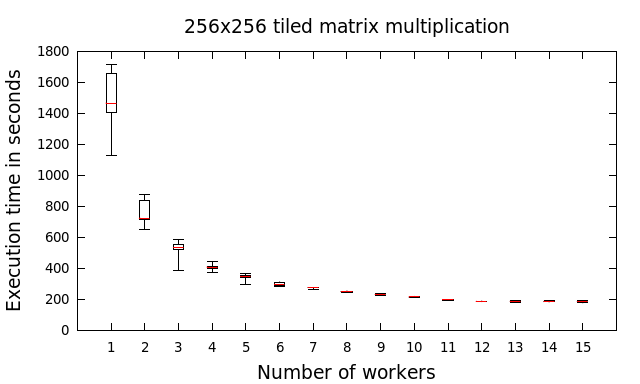
\includegraphics[width=90mm,natwidth=640,natheight=384]{tiledmul_250_100_256x256.png}
  \caption[TMM execution times for a matrix size of 256$\times$256]{TMM execution times for a matrix size of 256$\times$256}
  \label{fig:tiledmul_250_100_256x256}
\end{figure}

All benchmark results demonstrate reduced AETs when the number of workers is increased. The biggest performance gains can be found when stepping from 1 to 2 workers. Further increases of parallel workers show varying success. ZDT-3 benchmark instances with 10 and 100 genomes don't seem to profit from more than 2 workers. The performance for genome sizes of 1000 and 10000 increases in the best case until 8 - 9 workers, although, the performance gains are very small. The TMM benchmarks on the other hand show remarkable AET decreases when the number of workers is increased up to 12 workers.

At this point a more in-depth discussion of the benchmark results is put back on purpose, it can be found in section \ref{chap:evaluation:influence} and \ref{chap:evaluation:speedup}. The correctness of the optimization results must be verified first, otherwise, the test problems could execute arbitrary computations and the benchmarks would be meaningless.

\subsection{Correctness of ZDT-3 results}
In the case of ZDT-3 the task was to find an approximation to the optimal Pareto Front (OPF). The computed Pareto Fronts (CPF) are compared to the OPF using the Hypervolume (HV) indicator \cite{zitzler1999multiobjective}. Table \ref{table:hypervolume} gives the results for the indicator, where the HV is computed as the median over all benchmarks for a given genome size. Higher HV values indicate a better CPF.

\begin{table}
  \centering
  \caption{Hypervolume results for ZDT-3 benchmark instances}
  \begin{tabular}{lrrrr}\toprule[2pt]
    Test Problem & Hypervolume \\ \midrule
    NSGA-II, 10 genomes & 0.515 \\
    NSGA-II, 100 genomes & 0.458 \\
    NSGA-II, 1000 genomes & 0.340 \\
    NSGA-II, 10000 genomes & 0.330 \\
  \end{tabular}
  \label{table:hypervolume}
\end{table}

One can see that HV decreases with the number of genomes. It is well known that ZDT-3 optimization is harder the larger the genome is. 10 genomes produce the best results with HV = 0.515. Manual comparison of a CPF (randomly chosen from the results with 10 genomes) show high similarities with OPF, as can be seen in fig. \ref{fig:pf-comparison}. It is therefore concluded that the ZDT-3 optimization results are correct.

\begin{figure}
  \centering
  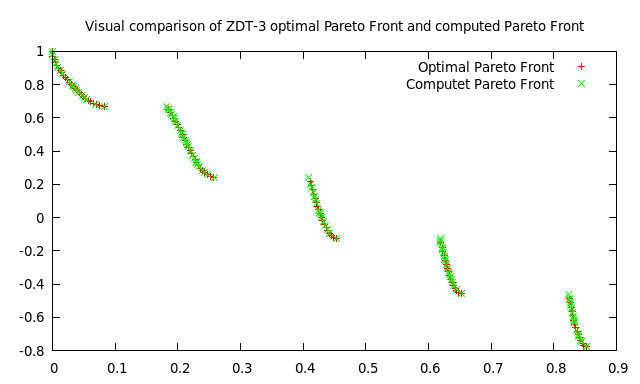
\includegraphics[width=110mm,natwidth=640,natheight=384]{pf-comparison.png}
  \caption[Comparison of optimal and computed PF for ZDT-3]{Visual comparison of ZDT-3 optimal Pareto Front and computed Pareto Front}
  \label{fig:pf-comparison}
\end{figure}

\subsection{Correctness of TMM results}
The goal of TMM optimization was to find tile sizes that reduce the computation time for a tiled matrix multiplication. Other than expected, the found tile sizes follow no recognizable pattern. The explanation is that the solution space is shallow which makes most solutions almost equally well suited. The exception are very small tile sizes with values less than 4.

The TMM optimization results were checked by executing a matrix multiplication with the optimized tile sizes and comparing the results to the execution time of the simple matrix multiplication (SMM). The results were twofold.

For 128$\times$128 matrix sizes, SMMs were faster by \unit[10]{\%} to \unit[15]{\%}. The reason is, that the additional nested loops of TMM and the consequent increased overhead is higher than the performance gain. Another reason is that 128$\times$128 matrices are small enough that sufficient parts of it fit into the L1 CPU caches to profit from the fast access rates.

In the case of 256$\times$256 benchmarks, all TMM executions were faster compared to the SMM by \unit[20]{\%} to \unit[30]{\%}. Additional experiments with larger matrices show that the performance gap between SMM and TMM increases with the matrix size. For example, 512$\times$512 matrix sizes provided about \unit[50]{\%} better performance for TMM. 1024$\times$1024 matrix sizes have about \unit[400]{\%} better performance. Again, the conclusion is that TMM benchmarks produce correct outputs.

\section{Performance Influencing Factors}
\label{chap:evaluation:influence}
Looking at the details of the benchmark results (presented in fig. \ref{fig:nsga_250_100_10} to \ref{fig:tiledmul_250_100_256x256}) two strange behaviours can be observed that need explanation. First, the AET for a benchmark with given setting (e.g. ZDT-3, 100 genomes, one worker) varies by a large amount. This is due to the influence of YARN, discussed in section \ref{chap:evaluation:influence-yarn}. Second, ZDT-3 benchmark instances for genome sizes of 10 and 100 experience AET reductions only up to 2 parallel workers, although the cluster provides more resources. The reason for this has been found to be the CPU saturation on Biohadoops master, discussed in section \ref{chap:evaluation:influence-cpu}. Other hard- and software influences on the benchmark results are summarized in section \ref{chap:evaluation:influence-other}. Their impact was not quantified.

It is difficult and a lot of work to find the reasons for performance degradations and strange phenomenas. This is especially true for a distributed environment like Hadoop. Further research could therefore focus on the development of distributed tracing and profiling tools, perhaps adapted to Hadoop. This would greatly simplify performance and bottleneck evaluations. Since Hadoop gains a lot of attraction also in business, it would be a good chance to bridge the gap between science and business.

\subsection{Influence of YARN}
\label{chap:evaluation:influence-yarn}
An interesting benchmark result is that the AETs for a given benchmark and setting vary by a large degree, e.g., ZDT-3 with 100 genomes and one worker. YARNs container placement and startup time was identified as the source of this variations.

The container placement of YARN has a big impact on AET. It defines on which machine a YARN container is allocated. If a worker container is executed on the same machine as the master container, they communicate without using the physical network. This effect brings a huge performance gain, as can be seen for example in figure \ref{fig:nsga_250_100_100}. In the single worker benchmarks, 4 out of 5 benchmarks executed with both the master and worker container running on the same machine. The result was a \unit[50]{\%} better performance (\unit[9.761]{s} average) compared to the fifth benchmark (\unit[14.164]{s}) where the master and worker were executed on different machines. Potential research projects could focus on a Hadoop scheduler that tries to put a YARN ApplicationMaster and its containers on the same machine to reliably produce similar results.

The number of worker containers running on the same machine as the master can also have a negative effect on AET. This is especially true if the master is already at the limit of the machines resources and must share them with the workers. An example for this can be found in figure \ref{fig:nsga_250_100_10} for 8 workers. Two worker containers were executed on the same machine as the master during 2 out of 5 benchmarks. The execution time results were \unit[87.977]{s} and \unit[88.014]{s}. In the remaining 3 benchmarks, only one worker container was executed on the same machine as the master, leaving more resources to the master. This results in execution times of \unit[68.423]{s} on average, a difference of more than \unit[20]{\%}.

Beside container placement, YARN influences AET through the container startup delay. Biohadoop can not use all of its configured workers until they are started by YARN (this is true for all YARN applications that use additional containers). An example of this phenomena can be found in the ZDT-3 benchmark instances with settings of 10 genomes and a single worker. In all five benchmarks for this setting, the master and worker container executed on different computers. Therefore, the results are comparable regarding the container placements. Nevertheless, the execution times vary from \unit[10.690]{s} to \unit[12.560]{s}, a difference of about \unit[15]{\%} due to delayed container allocations.

\subsection{CPU utilization}
\label{chap:evaluation:influence-cpu}
The results for ZDT-3 benchmark instances with genome sizes of 10 and 100 show no significant AET reductions for more than two workers (see fig. \ref{fig:nsga_250_100_10} and \ref{fig:nsga_250_100_100}). The reason for this odd behaviour is that the CPU running Biohadoops master is fully utilized when two ore more parallel workers are used.

This was established by measuring the CPU usage of the master during the execution of the benchmarks using Javas \texttt{OperatingSystemMXBean}\footnote{\url{https://docs.oracle.com/javase/7/docs/jre/api/management/extension/com/sun/management/OperatingSystemMXBean.html} last access: 27.01.2015}. The measurement was performed at an interval of \unit[1]{s}. Figure \ref{fig:cpu_10_100} shows the example CPU loads for ZDT-3 with 10 and 100 genomes executing with 3 workers.

\begin{figure}
  \centering
  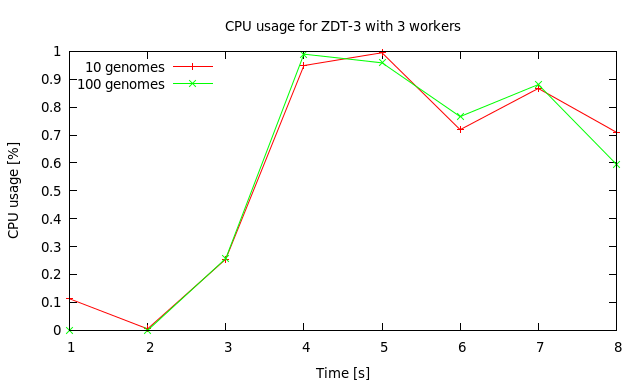
\includegraphics[width=90mm,natwidth=640,natheight=384]{cpu_10_100.png}
  \caption[CPU usage for ZDT-3, 10 and 100 genomes, 3 workers]{CPU usage for ZDT-3, 10 and 100 genomes, 3 workers - 250 iterations}
  \label{fig:cpu_10_100}
\end{figure}

It is arguable that the AET of ZDT-3 with 10 and 100 genomes is to short to get correct informations about the CPU usage. Therefore, the ZDT-3 benchmarks for 3 workers with 10 and 100 genomes were performed for 1000 iterations (original benchmarks iterate only 250 times). The results can be seen in fig. \ref{fig:cpu_10_100-1000-iter}. They confirm the CPU saturation for ZDT-3 with 10 and 100 genomes and three and more workers.

\begin{figure}
  \centering
  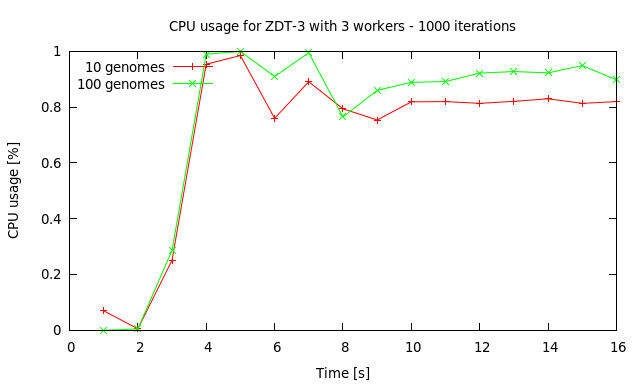
\includegraphics[width=90mm,natwidth=640,natheight=384]{cpu_10_100-1000-iter.png}
  \caption[CPU usage for ZDT-3, 10 and 100 genomes, 3 workers]{CPU usage for ZDT-3, 10 and 100 genomes, 3 workers - 1000 iterations}
  \label{fig:cpu_10_100-1000-iter}
\end{figure}

Since the master executes the sequential parts of the algorithms and in addition has to communicate with all workers, it is clear that a saturation of the master CPU prevents further performance gains. The problem worsens when additional YARN containers run on the computer that executes the master.

\subsection{Other influences}
\label{chap:evaluation:influence-other}
YARN and the CPU had the biggest effects on the benchmark results. In the following, other possible influencing factors are summarized. Their impact on the benchmark results is not quantified, as their correct evaluation is not trivial but very work intensive. As already mentioned, further research projects could develop tools to simplify this process.

\begin{description}
  \item [Network]: The network influences the benchmark results, as the master and its workers exchange messages through it. This influence is apparent in cases where YARN places its containers on the same computer, which can result in greatly reduced AETs. Nevertheless, the network influence is consistent: throughput and latency don't change over the time on the used test cluster.
  \item [RAM]: All benchmarks start with \unit[256]{MB} of Java heap memory which is enough for the containers to execute without causing excessive garbage collections. This was established by using the tool jvisualvm\footnote{\url{https://visualvm.java.net/} last access: 26.01.2015} (delivered with Java) for the ZDT-3 benchmark instance with 10000 genomes and the TMM with a matrix size of 256$\times$256. The memory usage for the master container is at about \unit[100]{MB} to \unit[150]{MB}. The memory usage for a worker is even lower and lies in the range of \unit[5]{MB} to \unit[30]{MB}. The conclusion is, that enough RAM was available during the benchmarks. To few RAM would have had significant impact on the performance.
  \item [CPU caches]: The CPU caches show their biggest influence during the TMM benchmarks. The workers execute matrix multiplications using provided tile sizes. If the tiles are small enough they fit into the L1 CPU cache which is the fastest memory available to a processor. Increased performance is the result. If the tiles don't fit into L1 cache, they need to be retrieved from L2 cache or even worse from main memory, which introduces latencies. Since TMM executes matrix multiplications to evaluate the fitness of an individual, the tile sizes affect the fitness evaluation of a single individual, and the whole runtime of the benchmark.
  \item [Java Java Just in Time Compiler (JIT)]: JIT\footnote{\url{https://en.wikipedia.org/wiki/Just-in-time_compilation} last access: 26.01.2015} compiles Java byte code into machine executable code that can be executed faster. During the benchmarks, JIT was set to optimize code parts that are executed more than 10000 times (this is the standard setting for the used Java Server runtime\footnote{\url{https://en.wikipedia.org/wiki/HotSpot} last access: 26.01.2015}). Small benchmarks, like ZDT-3 with 10 genomes, hit this threshold later in their execution. Therefore, the share of executed un-optimized code is larger compared to large benchmarks, e.g., ZDT-3 with 10000 genomes. This problem worsens with increasing numbers of workers.
  \item [Operating system (OS)]: The OS provides the basis for application execution. It provides also the interfaces for hardware usage, e.g. network communication. Therefore, it has large influence on executed applications. Using the right drivers and OS settings, e.g., for buffers, influence the performance of running applications significantly.
  \item [Building blocks]: Biohadoop uses Netty and Kryo for the communication between the master and its workers. Those libraries can be configured in many different ways. Again, the right configuration can provide performance increases or degradations.
\end{description}

\section{Speedup}
\label{chap:evaluation:speedup}
Speedup is a metric that tells how many times a parallel version of an algorithm (or system) runs faster compared to the sequential version. In the following, the maximum achievable speedups and the experimental speedup, i.e., the speedup achieved in the benchmarks, are presented in section \ref{chap:evaluation:max_speedup} and \ref{chap:evaluation:exp_speedup}, respectively.

\subsection{Maximum achievable Speedup}
\label{chap:evaluation:max_speedup}
The max. achievable speedup ($S_{max}$) for a given problem is the best-case result achievable through parallelization. It is computed using Amdahl's law \cite{amdahl1967validity}:

\begin{equation}
S_{max} = T / (T - t_p)
\end{equation}

In this formula, $T$ is the sequential execution time of an algorithm. During this sequential execution it is also measured how much time is spent in code parts that could be executed in parallel. This amount of time is defined as $t_p$.

The values for $T$ and $t_p$ are taken from the benchmark executions with a single worker. Since the measured AET for a given benchmark and one worker differs largely (e.g. ZDT-3 with 100 genomes), lower and upper max. achievable speedup boundaries are computed. The lower bound is computed using the worst sequential-to-parallel execution time ratio of a sequential benchmark run. The upper bound reflects the best sequential-to-parallel ratio. This proceeding gives more details over the achievable speedups.

Table \ref{table:achievable_speedups} presents the lower and upper bounds for the max. achievable speedups based on the benchmark results. The calculations show that ZDT-3 is generally not well suited for parallelization. In the best case with 1000 workers its performance can be increased by a factor of about 20 (upper bound). In the worst case with 10 genomes the performance can be increased by a factor of 5 (lower bound). The reason for the small achievable speedups is the bad sequential-to-parallel execution time ratio. ZDT-3 as fitness function is barely compute intense. As the fitness function is usually (but not in this case) the most compute intense part of an optimization, this leads to the mentioned bad sequential-to-parallel execution time ratio.

\begin{table}
  \centering
  \caption{Lower and upper bounds for max. achievable speedups}
  \begin{tabular}{lrrrr}\toprule[2pt]
    Test Problem & \parbox[r]{3.5cm}{Lower Achievable Speedup Boundary}& \parbox[r]{3.5cm}{Upper Achievable Speedup Boundary}\\ \midrule
    NSGA-II, 10 genomes & 4.816 & 11.046 \\
    NSGA-II, 100 genomes & 5.228 & 9.398 \\
    NSGA-II, 1000 genomes & 9.438 & 20.275 \\
    NSGA-II, 10000 genomes & 8.861 & 17.081 \\
    TMM, 128$\times$128 & 63.649 & 134.404 \\
    TMM, 256$\times$256 & 139.685 & 271.925 \\ \bottomrule[2pt]
  \end{tabular}
  \label{table:achievable_speedups}
\end{table}

TMM on the other side shows better results. It demonstrates that the test problem is well suited for parallelization. This is not surprising, as the parallel part in form of the fitness evaluation consists of a matrix multiplication which is known to be compute intensive. Therefore, the sequential-to-parallel execution time ratio is advantageous and opens the possibility to achieve good experimental speedups.

\subsection{Experimental Speedup}
\label{chap:evaluation:exp_speedup}
To compute the experimental speedup $S$ for a given benchmark, its sequential ($T_S$) and parallel ($T_P$) execution times are needed. $T_S$ is the execution time for a benchmark with a single worker. $T_P$ is the execution time for a benchmark with $P$ workers. $S$ is then calculated using the following formula \cite{hennessy2012computer}:

\begin{equation}
S = T_S / T_P
\end{equation}

Since the execution times for a given benchmark and setting vary often in a broad range, the lower and upper speedup boundaries for a given benchmark are computed. This is the same proceeding used for the computation of the max. achievable speedups. The boundaries are computed by using the min. and max. execution times for $T_S$ and $T_P$, respectively. For example, min. $T_S$ and max. $T_P$ of a given benchmark and setting are used to compute the lower speedup boundary. Max. $T_S$ and min. $T_P$ are used to compute the upper speedup boundary.

Fig. \ref{fig:speedup_min} shows the lower speedup bounds for all benchmarks, fig. \ref{fig:speedup_max} the upper speedup bounds. The figures demonstrate that the speedups for ZDT-3 benchmark instances are small. Even when looking at the best case of upper bound speedups it is clear that ZDT-3 takes little profit of the parallelization. The lower bounds of the experimental speedups show even poorer results. This comes at no surprise, since the max. achievable speedups computed in section \ref{chap:evaluation:max_speedup} are already small and it is very unlikely to reach them in practice.

\begin{figure}
  \centering
  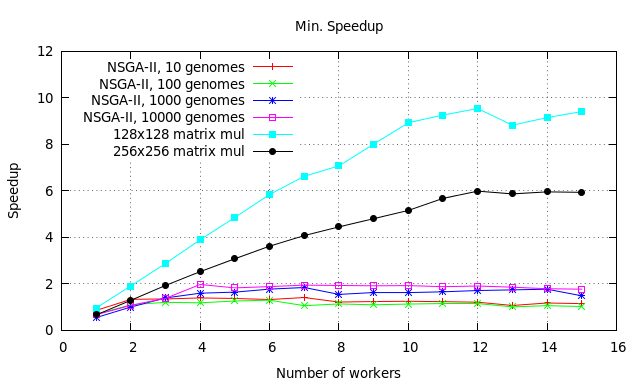
\includegraphics[width=100mm,natwidth=640,natheight=384]{speedup_min.png}
  \caption[Lower speedup boundaries for ZDT-3 and TMM benchmarks]{Lower speedup boundaries for ZDT-3 and TMM benchmarks}
  \label{fig:speedup_min}
\end{figure}
\begin{figure}
  \centering
  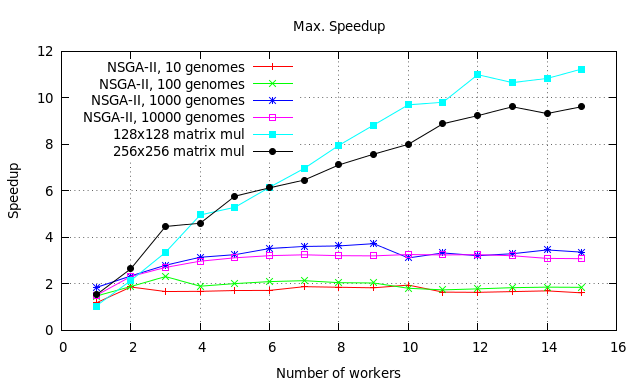
\includegraphics[width=100mm,natwidth=640,natheight=384]{speedup_max.png}
  \caption[Upper speedup boundaries for ZDT-3 and TMM benchmarks]{Upper speedup boundaries for ZDT-3 and TMM benchmarks}
  \label{fig:speedup_max}
\end{figure}

In contrast, the TMM results show good speedup behaviours. The benchmarks with a matrix size of 128$\times$128 demonstrate almost linear performance increases, which tend to be super-linear for the upper bound speedups. Super-linear speedups are usually suspicious. In this case they can be explained by the way the boundaries of the experimental speedups are computed. Nevertheless, also the lower bounds for TMM benchmarks with a matrix size of 128$\times$128 show almost linear increases. All speedups of all TMM benchmarks reach their maximum when 10 to 12 workers are used. This observation matches with the fact, that the whole cluster provides 12 cores.

The reason for the worse speedup of 256$\times$256 TMM compared to the 128$\times$128 version lies in the bigger solution space of 256$\times$256 TMM. It is more likely to find bad performing tile sizes for bigger matrices. The L1 cache sizes are limited and to big tile sizes affect the performance negatively.

The conclusion of the speedup results is that the parallelized search for values that minimize the ZDT-3 function is not well suited for Biohadoop --- at least for the used implementation. More advanced implementations may influence the sequential-to-parallel ratio and achieve better results. A different, more compute intense fitness function may also entail better speedup results. TMM on the other side provides good speedups and decrease the AET by a large amount. The parallelized search for optimal tile sizes using Biohadoop is favorable.

\section{Comparison to Standalone Implementations}
\label{chap:evaluation:comparison}
Standalone, sequential benchmarks ($SB$) of the test problems in section \ref{chap:evaluation:testproblems} are executed to determine if the algorithm parallelization using Biohadoop is advantageous. $SB$ are written in Java and executed on a single cluster machine. They use the same algorithm implementations and settings as the parallel versions, but run without Biohadoop and its task system. This entails that they perform no network communication at all.

Table \ref{table:sequential-runtimes} shows the fastest standalone sequential execution times ($T_S$), together with the fastest execution times achieved with parallel implementations ($T_P$). It provides also information about the speedup gained through parallelization. This speedup is computed the same way as in section \ref{chap:evaluation:exp_speedup}. The speedup is abbreviated with letter $G$ (gain) for better distinction to the previous results:

\begin{equation}
G = T_S / T_P 
\end{equation}

If $G$ is smaller than 1, the parallelization has a negative effect and should be avoided. In this cases, the parallel execution takes longer than the sequential execution. Values for $G$ that are bigger than 1 are favorable, since they provide reduced execution times.

\begin{table}
  \centering
  \caption[Execution times for standalone sequential implementations]{Execution times for $SB$}
  \begin{tabular}{lrrr}\toprule[2pt]
    Test Problem &  Standalone [s] & Parallel [s] & Performance gain \\ \midrule
    NSGA-II, 10 genomes & 2.852 & 6.461 & 0.441 \\
    NSGA-II, 100 genomes & 2.956 & 6.128 & 0.482 \\
    NSGA-II, 1000 genomes & 7.673 & 8.330 & 0.921 \\
    NSGA-II, 10000 genomes & 71.390 & 53.706 & 1.329 \\
    TMM, 128$\times$128 & 132.066 & 18.386 & 7.183 \\
    TMM, 256$\times$256 & 1500.705 & 178.158 & 8.423 \\ \bottomrule[2pt]
  \end{tabular}
  \label{table:sequential-runtimes}
\end{table}

The ZDT-3 benchmark instances for genome sizes up to 1000 show that the parallelization has a negative impact, the parallel execution times are bigger than the serial execution times. In this cases, it is better to stick with the serial implementation. ZDT-3 with a genome size of 10000 shows that the execution of parallel versions provide advantages in terms of execution time, although the performance gains are not very big.

The situation is completely different for the TMM benchmarks. The parallel implementations provide large benefits compared to the sequential versions.